\section{CP Violation in the \texorpdfstring{\BstoJpsiphi{}}{Bs0->Jpsiphi} Decay}
\label{sec:intro_Jpsiphi}

%%%%%%%%%%%%%%%%%%%%%%%%%%%%%%%%%%%%%%%%%%%%%%%%%%%%%%%%%%%%%%%
\subsection{The \texorpdfstring{\BsBsbar{}}{Bs0-Bs0bar} System}
\label{subsec:intro_Jpsiphi_Bs}
%%%%%%%%%%%%%%%%%%%%%%%%%%%%%%%%%%%%%%%%%%%%%%%%%%%%%%%%%%%%%%%

The $\Bs$ meson is a QCD bound state of an anti-b quark and an s quark. Its antiparticle is the $\Bsbar$ meson (b and anti-s). The $\Bs$
and the $\Bsbar$ are charge-neutral particles with an identical mass, which makes it possible to convert one into the other.
Figure~\ref{fig:mixing} shows the box diagrams that dominate the transition from $\Bs$ to $\Bsbar$. There are equivalent diagrams for the
opposite transition.
\begin{figure}[hbt]
  \centering
  \begin{subfigure}{0.5\textwidth}
    \centering
    \documentclass[11pt]{standalone}
\usepackage{color}
\usepackage[cmyk]{xcolor}
\usepackage{feynmp}
\usepackage{graphicx}
\usepackage{amsmath}
\usepackage{libertine}
\DeclareGraphicsRule{*}{mps}{*}{}

\newcommand{\Bs}{\text{B}_\text{s}^\text{0}}
\newcommand{\Bsbar}{\kern 0.06em \overline{\kern -0.06em \Bs \kern -0.32em} \kern 0.32em}

\begin{document}
\sffamily
\begin{fmffile}{./box1}
  \fmfframe(19,3)(17,3){
    \begin{fmfgraph*}(115,75)
      \fmfbottom{i1,d1,o1}%dummy vertex
      \fmftop{i2,d2,o2}
      \fmf{fermion,label=s,l.side=left}{i1,v1}
      \fmf{fermion,label={t,,c,,u},l.side=left}{v1,v2}
      \fmf{fermion,label=b,l.side=left}{v2,o1}
      \fmf{fermion,label=b,l.side=left}{v3,i2}
      \fmf{fermion,label={t,,c,,u},l.side=left}{v4,v3}
      \fmf{fermion,label=s,l.side=left}{o2,v4}
      \fmffreeze
      \fmf{boson,label=W,l.side=left}{v1,v3}
      \fmf{boson,label=W,l.side=right}{v2,v4}
      \fmf{plain,left=0.2}{o1,o2}
      \fmf{plain,left=0.2,label=$\Bsbar$}{o2,o1}
      \fmf{plain,left=0.2}{i2,i1}
      \fmf{plain,left=0.2,label=$\Bs$}{i1,i2}
    \end{fmfgraph*}
  }
\end{fmffile}
\end{document}

    \label{fig:mixing_1}
  \end{subfigure}%
  \begin{subfigure}{0.5\textwidth}
    \centering
    \documentclass[11pt]{standalone}
\usepackage{color}
\usepackage[cmyk]{xcolor}
\usepackage{feynmp}
\usepackage{graphicx}
\usepackage{amsmath}
\usepackage{libertine}
\DeclareGraphicsRule{*}{mps}{*}{}

\newcommand{\Bs}{\text{B}_\text{s}^\text{0}}
\newcommand{\Bsbar}{\kern 0.06em \overline{\kern -0.06em \Bs \kern -0.32em} \kern 0.32em}

\begin{document}
\sffamily
\begin{fmffile}{./box2}
  \fmfframe(19,3)(17,3){
    \begin{fmfgraph*}(115,75)
      \fmfbottom{i1,d1,o1}%dummy vertex
      \fmftop{i2,d2,o2}
      \fmf{fermion,label=s,l.side=left}{i1,v1}
      \fmf{fermion,label=b,l.side=left}{v2,o1}
      \fmf{fermion,label=b,l.side=left}{v3,i2}
      \fmf{fermion,label=s,l.side=left}{o2,v4}
      \fmf{boson,label=W$^-$,l.side=left}{v1,v2}
      \fmf{boson,label=W$^+$,l.side=left}{v4,v3}
      \fmffreeze
      \fmf{fermion,label={t,,c,,u},l.side=left}{v4,v2}
      \fmf{fermion,label={t,,c,,u},l.side=left}{v1,v3}
      \fmf{plain,left=0.2}{o1,o2}
      \fmf{plain,left=0.2,label=$\Bsbar$}{o2,o1}
      \fmf{plain,left=0.2}{i2,i1}
      \fmf{plain,left=0.2,label=$\Bs$}{i1,i2}
    \end{fmfgraph*}
  }
\end{fmffile}
\end{document}

    \label{fig:mixing_2}
  \end{subfigure}
  \caption{Dominant \BsBsbar{} mixing diagrams \cite{LHCb-PAPER-2013-002}.}
  \label{fig:mixing}
\end{figure}

Their mixing makes the $\Bs$ and $\Bsbar$ a coupled system of particles. The system comprises two eigenstates with different masses and
mean lifetimes (see Section~\ref{sec:pheno_mix}). A particle that is created as $\Bs$ can be observed as either a $\Bs$ or a $\Bsbar$ some
time later. As a result, the distribution of the time at which the \BsBsbar{} system decays is not a simple exponential, like it is for a
single particle.

The \emph{decay time} is defined as the time difference between the production and the decay of a particle in its rest frame. In
Section~\ref{sec:pheno_mix} the exact shape of the decay-time dependence of the \BsBsbar{} system will be discussed. The applied formalism
is common to the $\Dmes$, $\Bd$ and $\Bs$ mesons and, to some extend, also the $\kaon$ meson, which all mix with their antiparticles.
Because the differential decay rate as a function of time contains sinusoidal terms, mixing is often referred to as ``meson oscillations''.

In the Standard Model, CP violation enters the mixing process through the CKM-matrix elements at W-boson vertices. Since for CP violation
interfering amplitudes with different weak and strong phases are required (Equation~\ref{eq:interference}), the box diagrams from
Figure~\ref{fig:mixing} are not sufficient. These amplitudes depend on the mass of the internal up-type quark, which makes the top-quark
contributions dominating and to good approximation only one weak phase from $(\Vts\Vtb[*])^2$ remains.

Whereas the diagrams in Figure~\ref{fig:mixing} contain loops with virtual particles, there are also \BsBsbar{} transitions with real
intermediate states into which both $\Bs$ and $\Bsbar$ can decay. These amplitudes with real states interfere with the virtual amplitudes
with different weak phases and cause \emph{CP violation in mixing}. This leads to different rates for the CP-conjugate processes
$\Bs\to\Bsbartofbar$ and $\Bsbar\to\Bstof$, where f is a state into which only $\Bs$ can decay and $\overline{\text{f}}$ the CP-conjugate
state into which only $\Bsbar$ can decay.

Because the virtual amplitudes dominate the mixing process, CP violation in mixing is very small for the \BsBsbar{} system. The asymmetry
%\footnote{The asymmetry between two quantities $A$ and $B$ is defined as the ratio of their difference and their sum: $\frac{A-B}{A+B}$.}
between the $\Bs\to\Bsbartofbar$ and $\Bsbar\to\Bstof$ processes due to CP violation in mixing is measured to be approximately one per cent
\cite{Amhis:2012bh}. This is compatible with no CP violation given the current experimental uncertainties.

Depending on the final state, there may also be different amplitudes contributing to the decay of the $\Bs$ meson. Also then
interference can lead to different decay rates, in this case for the $\Bstof$ and $\Bsbartofbar$ processes. This form is termed \emph{CP
violation in decay}.

The first significant observation of CP violation in the $\Bs$ system was recently by LHCb \cite{LHCb-PAPER-2013-018}. This was a
measurement of CP violation in decay for $\Bsbar\to\Kp\pimes[-]$ and $\Bs\to\Km\pimes[+]$, where an asymmetry in the decay rates of about
30\% was found.

\newcommand{\ffig}{\fp}
\newcommand{\phimixfig}{\phi_\text{mix}}
\newcommand{\phifig}{\phi_\text{dec}}
\newcommand{\phibarfig}{\kern 0.15em \overline{\kern -0.15em \phi_\text{dec} \kern -0.60em} \kern 0.60em}
\begin{figure}[tb]
  \centering
  \resizebox{0.32\textwidth}{!}{\input{graphics/intro/decay.pdftex_t}}
  \caption{Interference between the $\Bstof[\fp]$ and $\Bs\to\Bsbartof[\fp]$ processes. The phases $\phimixfig$, $\phifig$, and
           $\phibarfig$ are the relevant weak phases contributing to the two decay paths from the mixing, $\Bs$ decay and $\Bsbar$ decay,
           respectively. This is assuming no CP violation in mixing or decay.}
  \label{fig:interference}
\end{figure}

An interesting situation occurs if both $\Bs$ and $\Bsbar$ can decay into the same final state $\fp$. In that case the processes
$\Bstof[\fp]$ and $\Bs\to\Bsbartof[\fp]$ interfere, which is depicted in Figure~\ref{fig:interference}. Even without CP
violation in mixing or decay, this interference may cause a difference between the rates of $\Bs(\to\Bsbar)\to\fp$ and
$\Bsbar(\to\Bs)\to\overline{\fp}$. This difference is called \emph{CP violation in the interference of decays with and decays without
mixing}.

A special case of this form of CP violation is the one where $\fp$ is a CP eigenstate. In this case $\fp$ and $\overline{\fp}$ are
identical and CP violation results in a difference between $\Bs(\to\Bsbar)\to\fp$ and $\Bsbar(\to\Bs)\to\fp$.

An example is the decay \BdtoJpsiKS, where $\Bd$--$\Bdbar$ mixing is implied. Assuming the Standard Model, a measurement of the
oscillations in its decay-time distribution yields the CKM angle $\beta$. This measurement was first performed by both the BaBar and Belle
experiments \cite{Aubert:2001nu,*Abe:2001xe}. The result of combining all currently available measurements of CP violation in this decay
\cite{Amhis:2012bh} is consistent with other measurements in the Standard Model framework \cite{Charles:2004jd,Bona:2005vz}.


%%%%%%%%%%%%%%%%%%%%%%%%%%%%%%%%%%%%%%%%%%%%%%%%%%%%%%%%%%%%%%%%
\subsection{\texorpdfstring{\BstoJpsiphi{}}{Bs0->Jpsiphi} Decay}
\label{subsec:intro_Jpsiphi_decay}
%%%%%%%%%%%%%%%%%%%%%%%%%%%%%%%%%%%%%%%%%%%%%%%%%%%%%%%%%%%%%%%%

The \BstoJpsiphi{} decay%
\footnote{Charge-conjugate particles, CP-conjugate decays and neutral-meson mixing will implied, unless stated otherwise.}
is one of the processes in the $\Bs$ system that is equivalent to the decay \BdtoJpsiKS{} in the $\Bd$ system. Its decay-time distribution
depends on the angle $\bs$ instead of $\beta$.

A complication arises from the fact that both the $\Jpsi$ and the $\phimesalt$ have a spin of one, which leads to three possible orbital
angular momentum configurations of the $\Jpsiphi$ system. This results in a superposition of three CP eigenstates, whereas there is only
one in \BdtoJpsiKS. Contributions of these states may be separated by an analysis of the $\Jpsi$ and $\phimesalt$ spin polarizations
\cite{Dighe:1995pd,*Dighe:1998vk}, which improves the sensitivity of the CP-violation measurement.

\begin{figure}[hbt]
  \centering
  \begin{subfigure}{0.5\textwidth}
    \centering
    \documentclass[11pt]{standalone}
\usepackage{color}
\usepackage[cmyk]{xcolor}
\usepackage{feynmp}
\usepackage{graphicx}
\usepackage{amsmath}
\usepackage{libertine}
\DeclareGraphicsRule{*}{mps}{*}{}

\newcommand{\Bs}{\text{B}_\text{s}^\text{0}}
\newcommand{\Bsbar}{\kern 0.06em \overline{\kern -0.06em \Bs \kern -0.32em} \kern 0.32em}

\begin{document}
\sffamily
\begin{fmffile}{./tree}
  \fmfframe(17,-25)(31,-25){
    \begin{fmfgraph*}(115,170)
      \fmfstraight
      \fmfleft{i0,i1,i2,i3,i4,i5}
      \fmfright{o0,o1,o2,o3,o4,o5}
      \fmf{fermion,tension=3.5,label.side=left,label=b}{v2,i3}
      \fmf{fermion,label=c,label.side=left}{o4,v2}
      \fmf{fermion,label=c,label.side=left}{v3,o3}
      \fmf{fermion,label=s,label.side=left,tension=2}{o2,v3}
      \fmf{boson,tension=2.4,label=W$^+$,label.side=right,right=0.3}{v2,v3}
      \fmffreeze
      \fmf{phantom,tension=0.3}{v2,v1,v3}
      \fmf{fermion,tension=0.5,label=s,label.side=left}{v1,o1}
      \fmf{fermion,tension=0.5,label.side=left,label=s}{i2,v1}
      \fmf{plain,right=0.2}{i2,i3}
      \fmf{plain,left=0.2,label=$\Bs$}{i2,i3}
      \fmf{plain,right=0.2}{o1,o2}
      \fmf{plain,left=0.2}{o1,o2}
      \fmf{plain,right=0.2}{o3,o4}
      \fmf{plain,left=0.2}{o3,o4}
    \end{fmfgraph*}
  }
\end{fmffile}
\end{document}

    \caption{}
    \label{fig:decay_tree}
  \end{subfigure}%
  \begin{subfigure}{0.5\textwidth}
    \centering
    \documentclass[11pt]{standalone}
\usepackage{color}
\usepackage[cmyk]{xcolor}
\usepackage{feynmp}
\usepackage{graphicx}
\usepackage{amsmath}
\usepackage{libertine}
\DeclareGraphicsRule{*}{mps}{*}{}

\newcommand{\Bs}{\text{B}_\text{s}^\text{0}}
\newcommand{\Bsbar}{\kern 0.06em \overline{\kern -0.06em \Bs \kern -0.32em} \kern 0.32em}

\begin{document}
\sffamily
\begin{fmffile}{./penguin}
  \fmfframe(17,-25)(31,-25){
    \begin{fmfgraph*}(115,170)
      \fmfstraight
      \fmfleft{i0,i1,i2,i3,i4,i5}
      \fmfright{o0,o1,o2,o3,o4,o5}
      \fmf{fermion,tension=1.8,label.side=left,label=b}{v5,i3}
      \fmf{fermion,tension=1.5,right=0.2,label.side=left,label={\hspace*{18pt}u,,c,,t}}{v2,v5}
      \fmf{gluon,tension=2}{v4,v2}
      \fmf{dbl_dashes,tension=0}{v4,v2}
      \fmf{fermion,tension=0.3,right=0.2,label.side=left }{v3,v2}
      \fmf{boson,tension=0.6,left=0.3,label=W$^+$,label.side=left}{v3,v5}
      \fmf{fermion,label=c,tension=0.9,right=0.3,label.side=left}{o4,v4}
      \fmf{fermion,label=c,tension=0.9,right=0.3,label.side=left}{v4,o3}
      \fmf{fermion,label=s,label.side=left}{o2,v3}
      \fmffreeze
      \fmf{fermion,tension=0.7,label=s,label.side=left}{v1,o1}
      \fmf{fermion,tension=1,label.side=left,label=s}{i2,v1}
      %\fmf{phantom,tension=0.4}{v4,v1}
      \fmf{phantom,tension=0.4}{v3,v1,v5}
      \fmf{plain,right=0.2}{i2,i3}
      \fmf{plain,left=0.2,label=$\Bs$}{i2,i3}
      \fmf{plain,right=0.2}{o1,o2}
      \fmf{plain,left=0.2}{o1,o2}
      \fmf{plain,right=0.2}{o3,o4}
      \fmf{plain,left=0.2}{o3,o4}
    \end{fmfgraph*}
  }
\end{fmffile}
\end{document}

    \caption{}
    \label{fig:decay_penguin}
  \end{subfigure}
  \caption{\BstoJpsiphi{} decay: (a) tree-level diagram; (b) penguin diagram \cite{LHCb-PAPER-2013-002}. The curled/dashed line in (b)
           represents a colour-neutral state, which can be a Z$^0$, a photon, or a colour-singlet gluon.}
  \label{fig:decay}
\end{figure}
Figure~\ref{fig:decay_tree} shows the dominant Standard Model contribution to the \BstoJpsiphi{} decay. This is a tree-level diagram,
where the $\qbar[b]$ quark decays into an $\qbar[s]$ quark and a c$\qbar[c]$ pair. The amplitude for this lowest order \emph{$\btoccs$
transition} is proportional to the CKM-matrix elements $\Vcs$ and $\Vcb[*]$.

The dominant contributions to the \BsBsbar{} mixing with internal top quarks (Figure~\ref{fig:mixing}) are proportional to
$(\Vts\Vtb[*])^2$. With the diagram from Figure~\ref{fig:decay_tree} this gives a weak phase difference between decays with and decays
without mixing of
\begin{equation}
  \label{eq:betasCKM}
  \begin{split}
    &\arg\left[(\Vts\Vtb[*])^2\right] + \arg\left(\Vcs[*]\Vcb\right) - \arg\left(\Vcs\Vcb[*]\right) \\
    &\qquad\qquad= 2\,\arg\left(-\frac{\Vts\Vtb[*]}{\Vcs\Vcb[*]}\right) = 2\bs
  \end{split}
\end{equation}

Additional contributions to the mixing and decay processes can affect the estimate of the weak phase. The quantity that is observed in a
measurement is $\phis$, which is equal to --2$\bs$ with the above assumptions.%
\footnote{There are various, often contradicting, notations of the phase difference in use. In this work $\bs$ is the CKM-triangle angle
(Equation~\ref{eq:bsAnglesDef}) and $\phis$ the observable in the decay-time distribution (see Section~\ref{sec:pheno_obs}). If only
dominant Standard Model contributions to both mixing and decay are considered, $\phis$ is equal to --2$\bs$.}

In the Standard Model, there are the mixing diagrams with real states and also higher order contributions to the decay, like the
\emph{penguin diagram} in Figure~\ref{fig:decay_penguin}. While the former are responsible for small Standard Model CP violation in mixing,
these amplitudes are not expected to contribute significantly to $\phis$ (see Section~\ref{sec:pheno_obs}). Although hard to estimate,
small contributions from penguin diagrams to the decay are expected \cite{Faller:2008gt,*Bhattacharya:2012ph}.

Beyond the Standard Model, modification of CP violation can come from new contributions to both the (virtual) \BsBsbar{} mixing process
\cite{Nir:1990hj,*Silverman:1998uj,*Ball:1999yi,*Dunietz:2000cr,Buras:2009if} and the $\Bs$ decay \cite{Chiang:2009ev,*Datta:2009fk}. In
previous measurements it was assumed that these contributions would be large, but only affecting $\phis$. This enables the use of a
simplified model for the decay-time distribution. It is now known that effects from non-Standard Model physics are small, which creates a
need for a more precise measurement that makes less assumptions. The model to be used in such a measurement is discussed in
Chapter~\ref{chap:pheno}.

Measurements of $\phis$ with the \BstoJpsiphi{} decay have been performed previously by the D0 \cite{Abazov:2011ry}, CDF
\cite{Aaltonen:2012ie}, \atlas{} \cite{Aad:2012kba,*ATLAS:2013nla}, and LHCb \cite{LHCb-PAPER-2013-002} experiments. The measurements and
their combination \cite{Amhis:2012bh} are compatible with no CP violation and also with the value of $\bs$ from the Standard Model fit
(Equations~\ref{eq:CKMAnglesCKMf} and \ref{eq:CKMAnglesUTf}). The LHCb measurement yielded
\begin{equation}
  \label{eq:phis1fb}
  \phis\text{\texteq+0.07\textpm0.09$\,$(stat.)\textpm0.01$\,$(syst.)~~rad\ ,}
\end{equation}
where the first uncertainty is statistical and the second systematic. This value is to be compared with the Standard Model estimate
--2$\bs$\texteq--0.0368$^\text{+0.0013}_\text{--0.0014}$\unitsp{}rad (see Equation~\ref{eq:CKMAnglesCKMf} and
reference~\cite{Charles:2004jd}).

A measurement of the decay-time distribution is not only sensitive to the phase $\phis$, but also to the lifetime parameters of the
\BsBsbar{} system. The decay-width average ($\Gs$\textequiv$\frac{\text{1}}{\taus}$, where $\taus$ is the mean lifetime) and difference
($\DGs$) of the two eigenstates were measured by D0, CDF, \atlas, and LHCb and also by CMS \cite{CMS:2012pca}.

In the Standard Model the parameter $\Gs$ is expected to be equal to the $\Bd$ decay width up to relative corrections of the order of
\tenpow{--3} \cite{Lenz:2006hd,*Lenz:2011ti}. $\Gd$ is measured to be 0.6583\textpm0.0030\unitsp\invps{} \cite{Amhis:2012bh}. A prediction
of the decay-width difference $\DGs$ yields 0.087\textpm0.021\unitsp\invps{} \cite{Lenz:2006hd,*Lenz:2011ti}. The measurements of $\Gs$ and
$\DGs$ and their combination \cite{Amhis:2012bh} are compatible with these predictions. The estimates from the LHCb measurement are given
by
\begin{subequations}
  \label{eq:width1fb}
  \begin{align}
    \label{eq:avWidth1fb}
    \Gs&\text{\texteq0.663\textpm0.005$\,$(stat.)\textpm0.006$\,$(syst.)~~\invps} \\
    \label{eq:diffWidth1fb}
    \DGs&\text{\texteq0.100\textpm0.016$\,$(stat.)\textpm0.003$\,$(syst.)~~\invps\ .}
  \end{align}
\end{subequations}

\begin{figure}[tb]
  \centering
  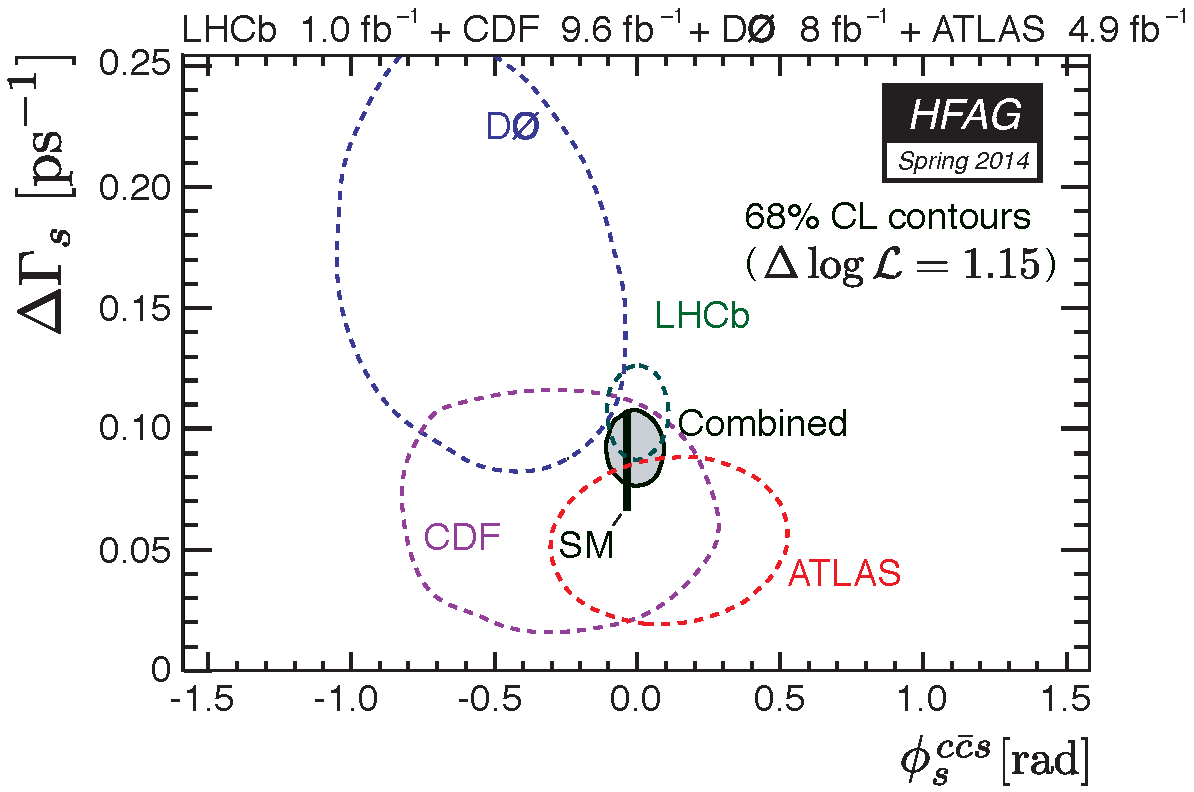
\includegraphics[width=0.7\textwidth]{graphics/intro/hfag_spr2014_DGsphis_comb-crop}
  \caption{Combination of $\phis$ (here represented as $\phisccs$) and $\DGs$ measurements by HFAG \cite{Amhis:2012bh}.
           The estimates at 68\% confidence level by the different experiments are shown by the dashed contours.
           Note that the LHCb contour is a combination of measurements in the \BstoJpsiphi{} and \BstoJpsipipi{} decays.
           The combined 68\% confidence region is shown by the shaded area and the Standard Model prediction by the vertical bar.}
  \label{fig:phisDGs}
\end{figure}

A graphical representation of the current status of $\phis$ and $\DGs$ measurements Heavy Flavour Averaging Group (HFAG) is shown in
Figure~\ref{fig:phisDGs}. Apart from the four \BstoJpsiphi{} measurements, also a $\phis$ measurement with the \BstoJpsipipi{} decay by
LHCb was included in the combination that is shown in this figure. The 68\% confidence-level (CL) contour of the combined result is
consistent with the region that represents the Standard Model prediction.


%%%%%%%%%%%%%%%%%%%%%%%%%%%%%%%%%%%%%%%%%%%%%%%%%%%%%%%%%%%%%%%%%%%
\subsection{The \texorpdfstring{$\mumuKK$}{mu+mu-K+K-} Final State}
\label{subsec:intro_Jpsiphi_final}
%%%%%%%%%%%%%%%%%%%%%%%%%%%%%%%%%%%%%%%%%%%%%%%%%%%%%%%%%%%%%%%%%%%

The $\Jpsiphi$ system is unstable and only its decay products can be detected. There are many possibilities for both the $\Jpsi$ and
$\phimesalt$ mesons to decay \cite{PDG2012}. The only final state that will be considered here is $\mumu\,\KK$, where the muon pair
originates from the $\Jpsi$ decay and the kaon pair from the $\phimesalt$ decay. All four particles can be detected efficiently by the LHCb
detector (see Section~\ref{sec:intro_LHCb}). Processes equivalent to \BstoJpsimumuphiKK{} often have larger decay rates, but lead to more
complicated final states that cannot be detected as efficiently.

Since the $\mumuKK$ final state can also be reached through resonances other than the $\Jpsi$ and the $\phimesalt$, interference with other
processes needs to be considered. To optimize for $\Jpsiphi$, a region in kinematic phase space is selected where this intermediate state
dominates.

The measured invariant mass of the muon pair is required to be between 3.03 and 3.15~\GeV{} (see also Section~\ref{sec:exp_selBkg}).%
\footnote{The unit of energy used in particle physics is the \emph{electronvolt} (eV), which is approximately equal to
1.6\tenpowmult{--19}~J. Derived units for momentum and mass are \eVc{} and \eV, respectively, where $c$ is the speed of light.}
This restriction is assumed to select only those \BstomumuKK{} decays with muons coming from a $\Jpsi$, which has a mass of approximately
3.10~\GeV{}~\cite{PDG2012}.

Also the invariant-mass range of the $\KK$ pair is restricted, but there the situation is more complicated. An analysis of the resonant
components in the $\KK$ system \cite{LHCb-PAPER-2012-040} has shown that there is a mass region where the $\phimes$ dominates, but other
contributions cannot be neglected.

\begin{figure}[tb]
  \centering
  %\begin{tikzpicture}[line width=0.08em]
  %  \node [anchor=south] {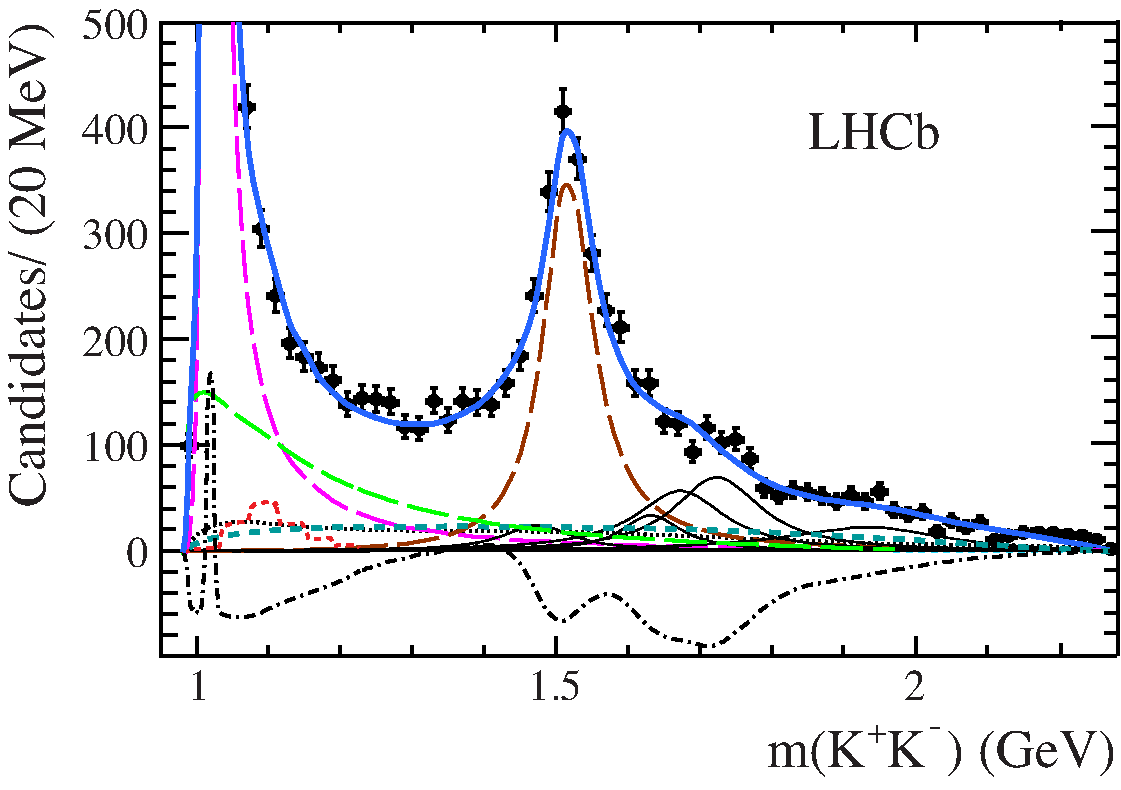
\includegraphics[width=0.7\textwidth]{graphics/intro/KKComponents}};
  %  \draw[red] (-0.2047\textwidth,0.04\textwidth) -- (-0.2047\textwidth,0.52\textwidth);
  %\end{tikzpicture}

  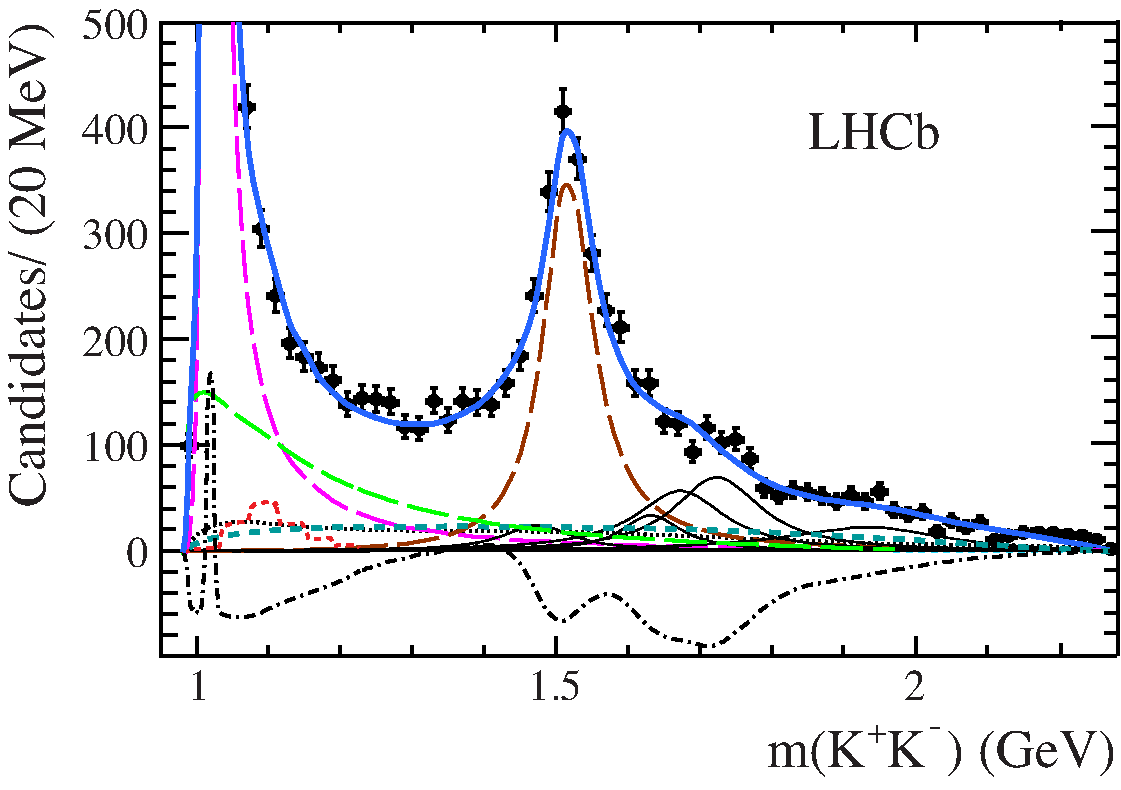
\includegraphics[width=0.7\textwidth]{graphics/intro/KKComponents}
  \caption{$\KK$-mass spectrum in \BstoJpsiKK{} decays \cite{LHCb-PAPER-2012-040}. The black points represent a histogram of decay
           candidates.
           %, where the size of the error bar shows the fluctuation expected from a Poisson distribution of the number of entries
           %in each mass bin.
           A model of the mass distribution is shown as the blue curve. The largest contributions to the distribution
           come from the $\phimes$, $\ftwop$, and $\fzero$ resonances, which are shown as the magenta,
           brown, and green long-dashed lines, respectively. Other resonances are shown as the thin, black curves and a non-resonant
           contribution as the dashed, cyan curve. Contributions from interference are represented by the dotted-dashed, black line. The
           small dotted, black and dashed, red contributions are backgrounds of four particles that do not originate from a \BstoJpsiKK{}
           decay.}
           %The region to the left of the vertical, red line is dominated by the $\phimes$.}
  \label{fig:KKComponents}
\end{figure}

The $\KK$-mass spectrum in \BstoJpsiKK{} decays is shown in Figure~\ref{fig:KKComponents}. The contribution of the $\phimes$ is represented
by the dashed, magenta curve. Note that part of the $\phimesalt$ peak is not visible because of the truncated vertical scale.

For the \BstoJpsiphi{} CP-violation measurement, only $\KK$ pairs with a mass between 0.99 and 1.05~\GeV{} are selected. In this region the
$\phimes$ clearly dominates, but there are also contributions from the $\fzero$ and from $\KK$ pairs that do not originate from the decay
of a resonance.

The $\KK$ system is in a state of zero orbital angular momentum for both of the additional contributions and hence they are referred to as
the \emph{$\KK$ S-wave}. Because the $\Jpsiphi$ and $\KK$ S-wave processes are observed simultaneously in a measurement, the analysed decay
is \BstoJpsiKK.

Because the $\phimes$ is a spin-one particle, the orbital angular momentum of the $\KK$ system has a P-wave configuration for the
$\Jpsiphi$ intermediate state. This makes the spatial distributions of the final-state particles different from the S-wave distributions,
which enables a statistical separation of these two components based on variables other than the $\KK$ mass. An analysis of the spatial
distributions also separates the three CP eigenstates of the $\Jpsiphi$ system, which is not possible with the $\KK$ mass.

The directions of the final-state particles are specified with respect to the directions of the $\mumu$ and $\KK$ momenta in the
centre-of-mass system of the $\Bs$ meson (see Section~\ref{sec:pheno_angles}). This is done with three \emph{decay angles}, which can be
computed given the four-momenta of the final-state particles. These angles are included in the model of the decay, in addition to the decay
time.
